
Figure~\ref{fig:structure} is the overview of this full-spectrum program adaptivity analysis.
% There are mainly three parts, each targeting on a challenge above.
It is composed of three parts, each targeting on a challenge above.
The fundamental part is the {\tt Query While} language designed for formalizing the 
adaptive data analysis. Building on this, 
the execution-based adaptivity analysis (formalization)
and the static program analysis for approximating the upper bound of the 
adaptivity are the two major analysis parts of this full-spectrum adaptivity analysis.
\begin{figure}
   \centering   
   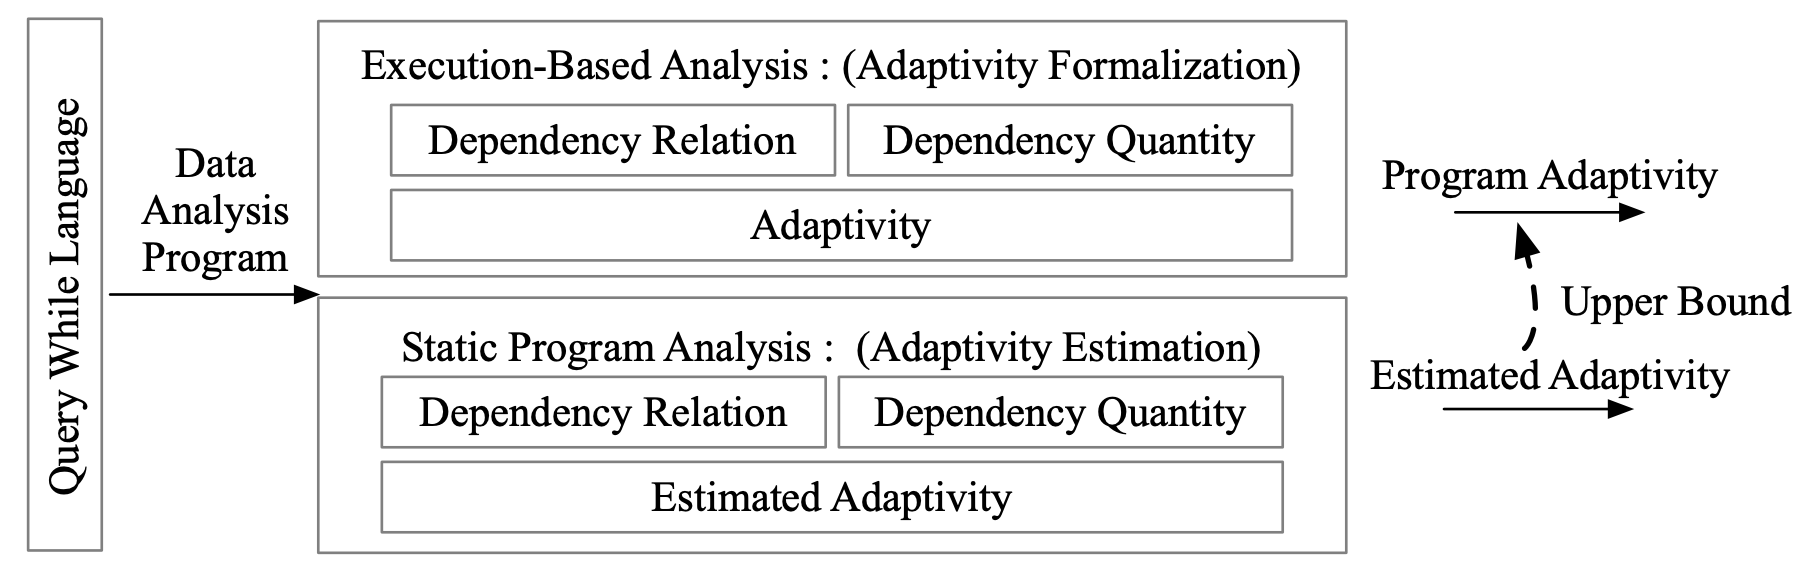
\includegraphics[width=1.0\textwidth]{figures/overview.png}
  \caption{High level architecture of the Program Analysis Framework for Adaptivity Analysis}
   \label{fig:structure}
\end{figure}